\section{Study 4: Wind Robustness}
\label{sec:study4}

Outdoor and warehouse-deployed throwing systems must operate under non-zero ambient
airflow.
This study extends the full \mcpilot{} pipeline to wind, tests whether an explicit
wind-conditioned policy outperforms a blind GP, and documents the curse-of-dimensionality
failure that occurs when the trial budget is insufficient for the expanded state space.

\subsection{Hit-Rate Threshold}
\label{sec:study4:threshold}

All wind experiments use the same 10\,cm hit radius as the other studies.
We do not relax the threshold for wind conditions; a 10\,cm target accepts landing
errors comparable to typical bin-mouth dimensions and is physically consistent
across all five studies.
This means wind results are directly comparable to the noise and height studies.

\subsection{Air-Relative Drag Correction}
\label{sec:study4:physics}

The baseline drag equation (Eq.~\ref{eq:drag}) uses absolute ball velocity
$\dot{\mathbf{p}}$.
Under wind $\mathbf{w}$, the physically correct formulation uses the air-relative
velocity $\mathbf{v}_{\mathrm{rel}} = \dot{\mathbf{p}} - \mathbf{w}$:
\begin{equation}
  \mathbf{F}_D = -\tfrac{1}{2}\rho\, C_D(\mathrm{Re})\, A\,
    \|\mathbf{v}_{\mathrm{rel}}\|\, \mathbf{v}_{\mathrm{rel}}, \quad
  \mathrm{Re} = \frac{\|\mathbf{v}_{\mathrm{rel}}\| \cdot 2r}{\nu}.
  \label{eq:wind_drag}
\end{equation}
This correction was applied to both the NumPy and PyBullet simulators.
A headwind ($\mathbf{w}$ opposing ball motion) decelerates the ball, reducing range;
a tailwind extends range.
For a 57\,g tennis ball at typical release speeds of 2--4\,m/s, a 5\,m/s headwind
deflects the landing position by $\approx 5$--15\,cm depending on target distance.

\subsection{State Augmentation: 8-D to 11-D}
\label{sec:study4:state}

The blind (wind-unaware) system uses the 8-D augmented state
$\tilde{\mathbf{x}} = [\mathbf{x},\, \mathbf{P}] \in \mathbb{R}^8$.
The wind-aware system appends the wind vector:
\begin{equation}
  \tilde{\mathbf{x}} =
    \underbrace{[x,\, y,\, z,\, v_x,\, v_y,\, v_z]}_{\text{ball state}}
    \oplus
    \underbrace{[w_x,\, w_y,\, w_z]}_{\text{wind}}
    \oplus
    \underbrace{[P_x,\, P_y]}_{\text{target}},
  \label{eq:wind_state}
\end{equation}
giving $\mathrm{STATE\_DIM} = 11$.
Wind is treated as task context: fixed per throw, carried forward unchanged through the
GP rollout so the model predicts velocity deltas conditioned on known $\mathbf{w}$.
The policy consumes both target and wind: $\pi_\theta(\mathbf{P},\, \mathbf{w})$,
expanding the RBF input from 2-D to 5-D (including $w_z$ for vertical gusts).

\subsection{Wind Models}
\label{sec:study4:windmodels}

Three physically distinct wind scenarios were implemented:

\paragraph{W1 — Constant wind.}
A fixed headwind vector $\mathbf{w} = (w_x, 0, 0)$ for the entire episode.
Four levels tested: calm ($\mathbf{w} = \mathbf{0}$, baseline reference), light
($w_x = 2.5$\,m/s), moderate ($w_x = 5.0$\,m/s), and strong ($w_x = 8.0$\,m/s).
The aware variant uses 5.0\,m/s.

\paragraph{W2 — Random gusts.}
Gusts arrive as a Poisson process; each gust has peak magnitude 4.0\,m/s and duration
$T_{\mathrm{gust}} = 0.15$\,s.
Each throw may experience a different number of gusts at different times.

\paragraph{W3 — Ornstein-Uhlenbeck turbulence.}
A continuous turbulence model with $\sigma = 4.0$\,m/s, mean $w_{\mathrm{mean}} = 0.3$\,m/s,
and correlation time $\tau = 1/\alpha = 1.43$\,s.
Turbulence provides correlated, time-varying disturbance that cannot be treated as
a fixed context.

\subsection{Results}
\label{sec:study4:results}

Table~\ref{tab:wind_results} and Figure~\ref{fig:wind_hitrates} report the full
9-configuration matrix, each run for 15 trials.

\begin{table}[t]
  \centering
  \caption{Wind robustness results (15 trials each).
           All blind models outperform their aware counterparts.
           Hit radius = 10\,cm (consistent with all other studies).}
  \label{tab:wind_results}
  \small
  \begin{tabular}{llcccc}
    \toprule
    Wind & Policy & Hits & Hit (\%) & Mean Err & Final \\
    Type &        &      &          & (cm)     & Cost \\
    \midrule
    No wind   & Blind & 11/15 & 73  & 10.3 & 0.315 \\
    W1 2.5m/s & Blind &  8/15 & 53  & 19.9 & 0.294 \\
    W1 5.0m/s & Blind &  8/15 & 53  & 22.0 & 0.262 \\
    W1 8.0m/s & Blind &  7/15 & 47  & 23.5 & 0.242 \\
    W1 5.0m/s & \textbf{Aware} &  7/15 & \textbf{47} & 24.6 & 0.292 \\
    \midrule
    W2 gusts  & Blind &  8/15 & 53  & 24.2 & 0.289 \\
    W2 gusts  & \textbf{Aware} &  6/15 & \textbf{40} & 28.2 & 0.331 \\
    \midrule
    W3 turb.  & Blind &  9/15 & \textbf{60}  & 17.0 & 0.287 \\
    W3 turb.  & \textbf{Aware} &  7/15 & \textbf{47} & 25.9 & 0.303 \\
    \bottomrule
  \end{tabular}
\end{table}

\paragraph{Constant wind is absorbed implicitly.}
The blind GP absorbs constant wind as a deterministic dynamics bias.
Performance degrades gracefully with wind strength: 73\% (no wind) $\to$ 53\% (2.5\,m/s)
$\to$ 53\% (5.0\,m/s) $\to$ 47\% (8.0\,m/s).
In constant-wind conditions the GP does not need an explicit wind input: it learns a
shifted speed-to-range mapping that incorporates the wind deflection.

\paragraph{The counterintuitive finding: blind beats aware in all conditions.}
The wind-aware model (5.0\,m/s W1) achieves only 47\% --- the same as the strong blind
baseline.
Under gusts, blind achieves 53\% while aware achieves 40\%.
Under turbulence, blind achieves 60\% while aware achieves 47\%.
In every configuration the blind model outperforms the aware model.

\paragraph{Root cause: curse of dimensionality.}
The 250 RBF policy centres distributed uniformly in the 2-D blind policy space
($P_x, P_y$) give $250^{1/2} \approx 15.8$ effective centres per dimension.
The same 250 centres in the 4-D aware policy space ($P_x, P_y, w_x, w_y$) give
$250^{1/4} \approx 3.98$ effective centres per dimension — exponentially sparser.
This means large gaps exist between policy centres in the wind dimensions; for any
wind value between two centres, the policy must extrapolate rather than interpolate.
With the same 1500 gradient steps per trial and 15 trials total, the aware policy
receives the same number of gradient updates but is trying to populate a 4-D manifold
with the density of a 2-D one.

This analysis is detailed in Section~\ref{sec:study4:dimscaling}.
Explicit wind conditioning is only beneficial when the trial budget scales with the
added policy dimensionality; empirically, this requires $\sim$40+ trials for a
4-D policy space.

\paragraph{RBF centre initialisation failure.}
An additional failure mode was identified in the aware models: if RBF centres are
initialised in a box that does not include the actual wind speed, all basis functions
have near-zero activation and the policy is permanently dead (observed: W1-aware
initial run, 0\% hit rate, 84.1\,cm mean error).
The fix applies the lengthscale scaling rule (Section~\ref{sec:convergence:lengthscale})
to the wind dimensions: centres span $[w - \epsilon,\, w + \epsilon]$ for constant wind
and $[-w_{\max},\, w_{\max}]$ for stochastic wind, with $\ell_w = 0.15 \times
2\,w_{\max}$.

\subsection{Sample-Efficiency Analysis}
\label{sec:study4:dimscaling}

The blind GP uses $N_b = 250$ RBF centres over a 2-D policy space.
Effective centre density scales as $N_b^{1/d}$ where $d$ is the policy dimension.
For the 2-D blind policy this gives $\approx 15.8$ centres/dimension; for the 4-D
aware policy, $\approx 3.98$ centres/dimension.

The practical consequence is that the aware policy requires $O(d^2)$ more data to
achieve the same generalisation quality.
Going from 2-D to 4-D policy requires $\approx 4 \times$ more trials, bringing the
effective minimum from $\approx 10$ to $\approx 40$ trials.
The 15-trial budget tested here sits squarely in the regime where the aware model is
underpowered.

\paragraph{Practical guidance.}
For deployment in constant or slowly-varying wind, treat wind as an implicit
environmental bias absorbed by the blind GP.
Invest in wind-aware models only when the trial budget exceeds
$\sim N_{\mathrm{trials,\,2D}} \times (d_{\mathrm{aware}}/2)^2$ and only after
verifying that RBF centres cover the actual wind range.

\begin{figure}[t]
  \centering
  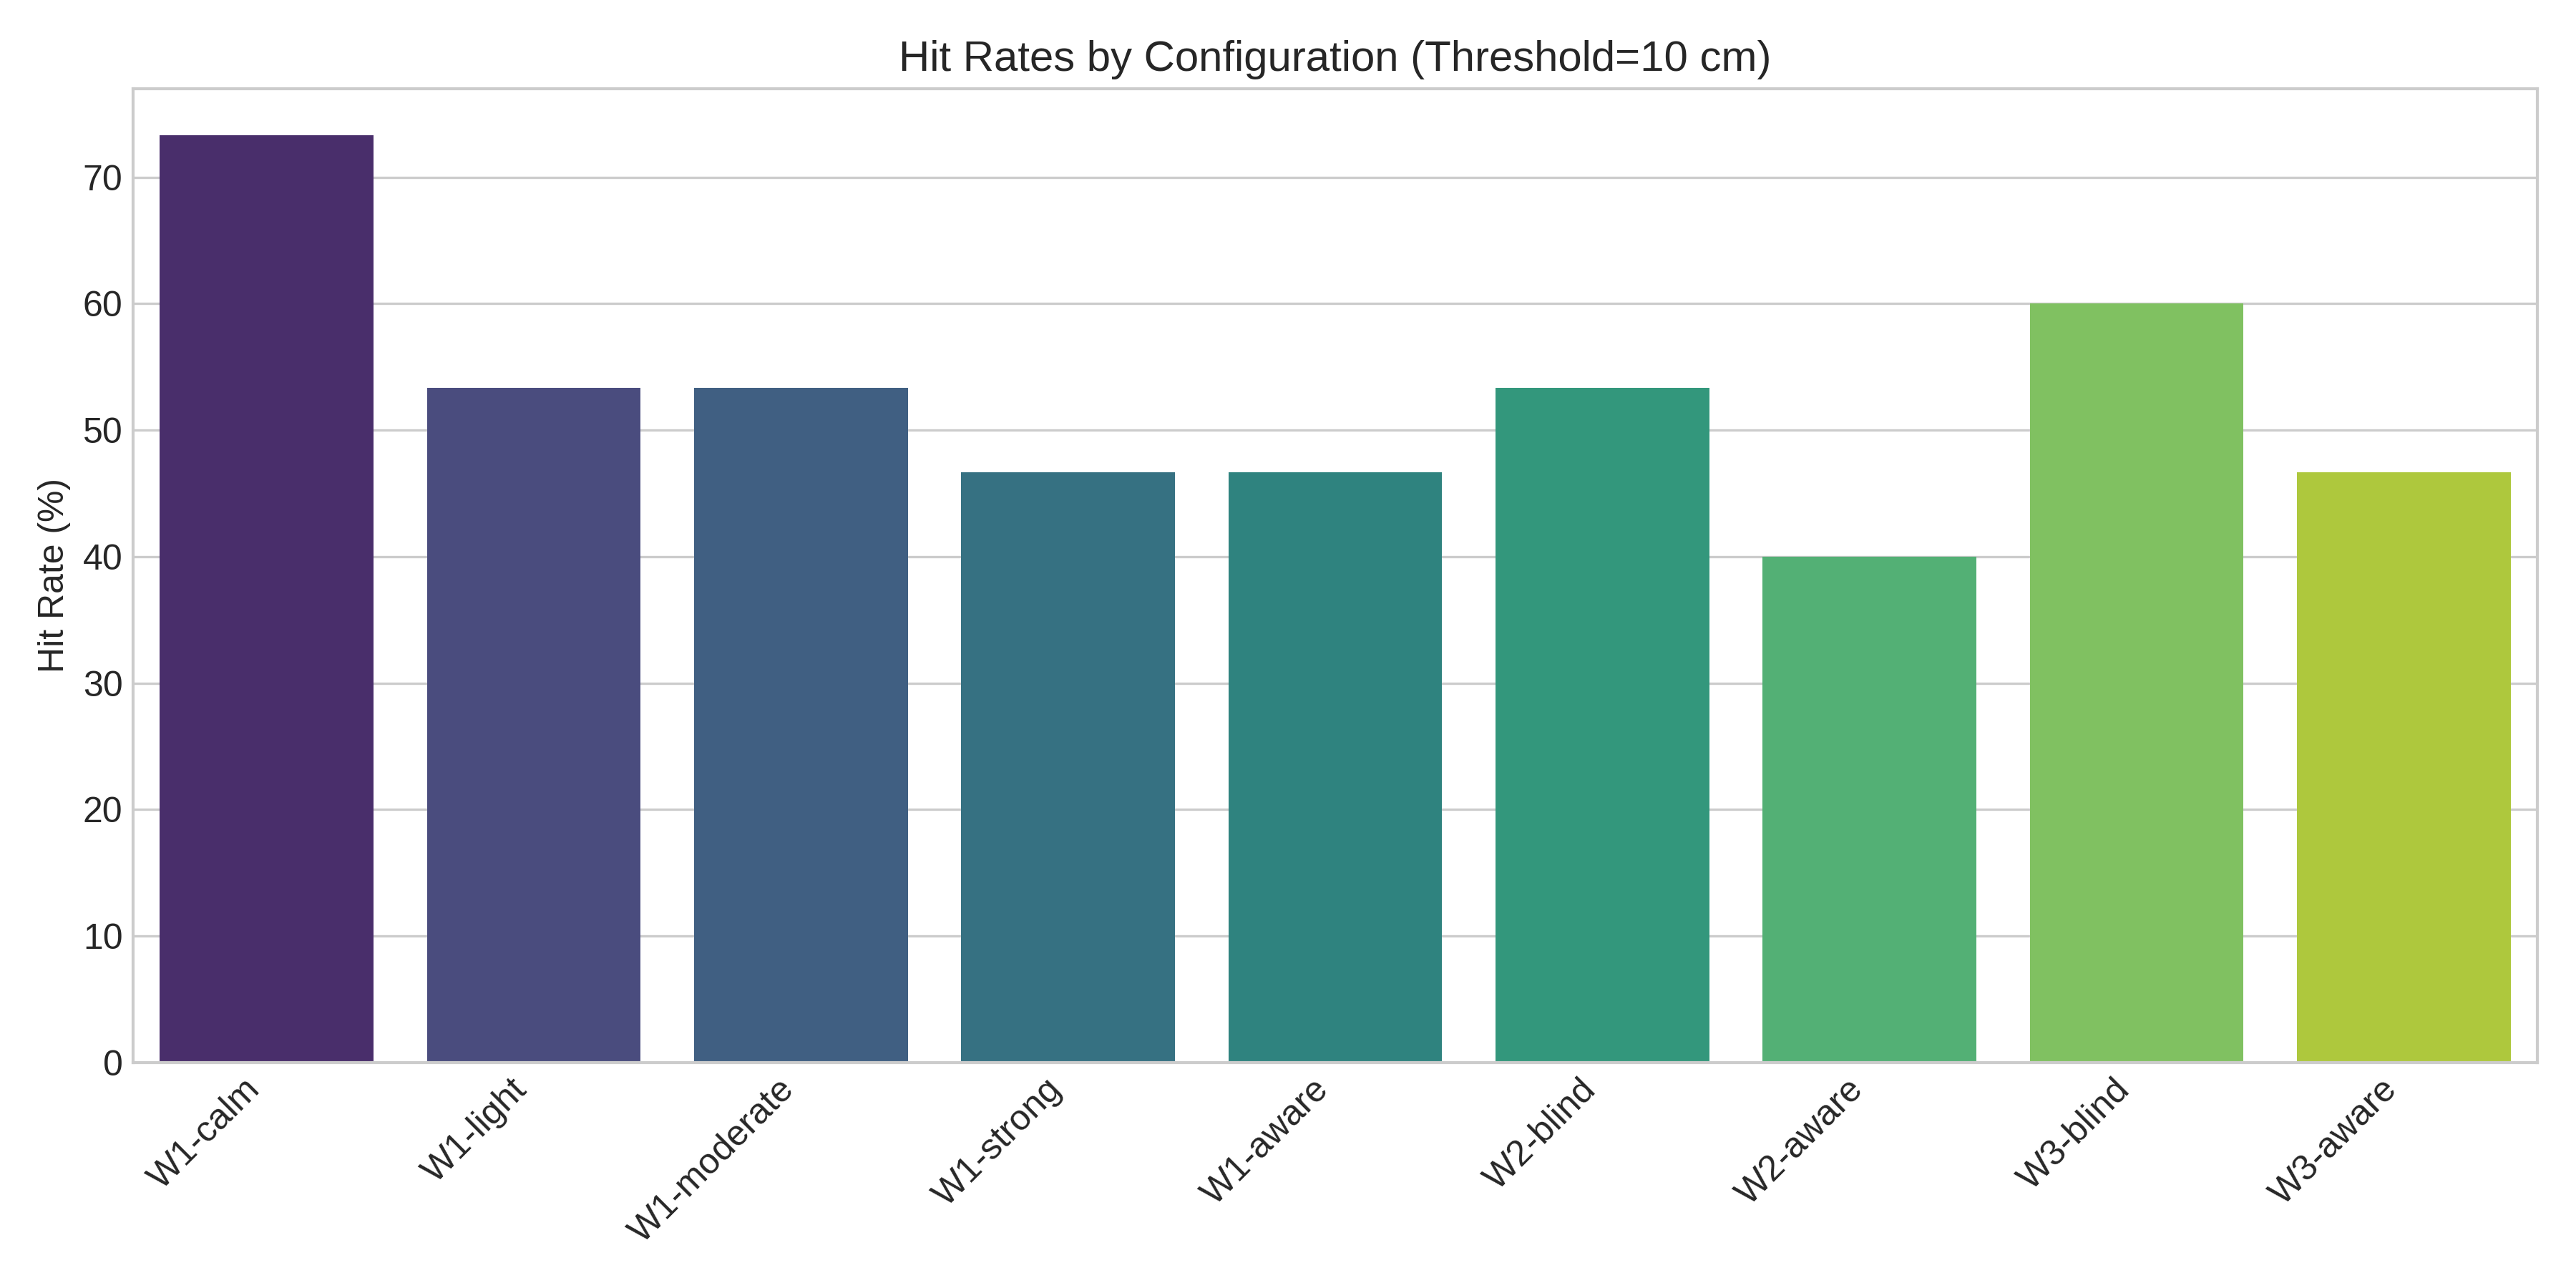
\includegraphics[width=\columnwidth]{../ppt/performance_analysis_plots/hit_rates.png}
  \caption{Hit rates across all 9 wind configurations.
           Blind models (solid) consistently outperform aware models (hatched) within
           the 15-trial budget.}
  \label{fig:wind_hitrates}
\end{figure}
